\chapter{Demodulator Benchmarking}
In order to compare the results of the different demodulators a method of benchmarking must be instituted. Each one of the demodulators was tested using multiple audio files that have different characteristics. These different files as well as the advantage of using them in the benchmarking are explained in their corresponding section. The winner of each of the benchmark files is determined by which demodulator could demodulate the most packets out of the file. It is worth noting that for each test audio file a sample rate of 48000Hz was standardized on since it works out nicely to 40 samples per bit period for 1200 baud digital communications. Although all the tests were performed with audio at a sample rate of 48000Hz, it is not expected that the results would change much if a different sample rate was chosen since sample rate dependent items are calculated from file meta data as opposed to hard coded constants to suit 48000Hz audio. 

\section{Plain, Straight, and Clean Packets}
These audio files were just what the title implies - straight packets. What is meant by straight packets is that they are pure "perfect" 1200Hz and 2200Hz tone audio samples. There is no noise introduced through artificial or natural means such as that introduced through the intrinsics of using RF. Although these files do not provide meaningful results for hardware or already implemented software solutions (since these devices should be able to decode every packet in the audio file) it still provides a good starting point for getting new algorithms up and running. Two of these clean files were generated. One was generated from an OpenTracker creating packets with a counter and the text "The quick brown fox jumps over the lazy dog". This audio file contained a total of 40 packets each separated by 30ms and proved to be short enough to allow for quick cross checking as modifications were made. The second file was generated in software using Toledo's javAX25 package. All that is relevant at this point is that it has perfect levels (1200Hz and 2200Hz tones are at the exact same level) and contains 200 packets each separated by 300ms making the file quite a bit longer. An sample from the 200 packet audio file can be seen in Figure \ref{gen200Segment}.
\begin{figure}
  \centering
	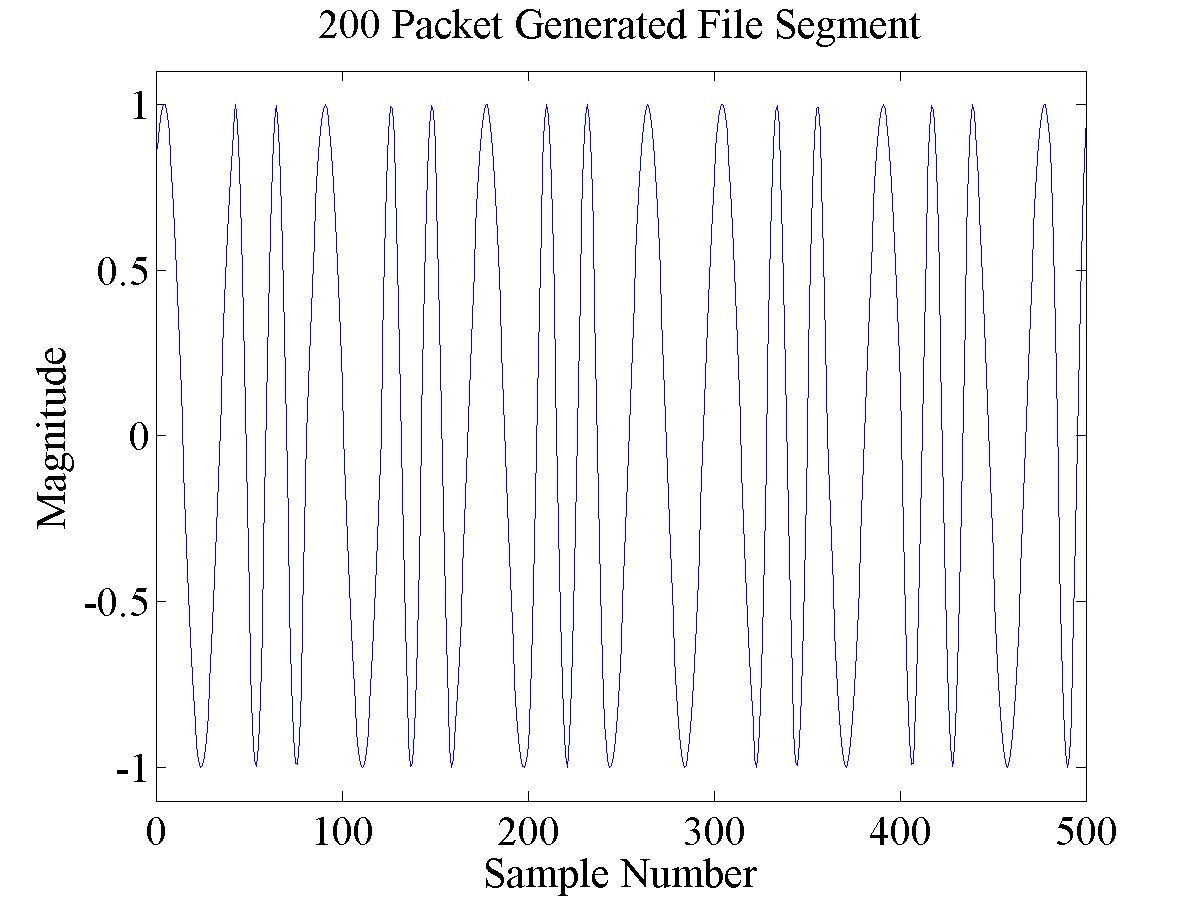
\includegraphics[width=0.75\linewidth]{images/200PacketGeneratedFileSegment.png} 
	\caption{Example of the AFSK signal present in the 200 packet generated file.}
   \label{gen200Segment}
\end{figure}

\section{White Noise Testing}
The second test file that was used on the demodulators was the 40 packet OpenTracker file mentioned in the previous section with added artificial white noise. An advantage of this file is that its contents are known, it contains 40 packets, while still being a reasonable benchmarking file because the later packets in the file are buried in noise. No demodulator could demodulate all the packets out of the file as the noise was increased all the way up to a signal to noise ratio (SNR) of 0.5, making the magnitude of the white noise twice that of the original signal. There were total of 10 steps of increasing noise meaning that at each noise level there were approximately 4 packets. This noise was added to the original audio file using the audio editing program Audacity\,\cite{Mazzoni}. Although this file does not directly characterize what is introduced by RF, it provides a reasonable test simulating the effects of a decreased SNR on the audio signal. An example segment from this white noise added file can be seen in Figure \ref{OT3TestwNoiseSegment}.
\begin{figure}
  \centering
	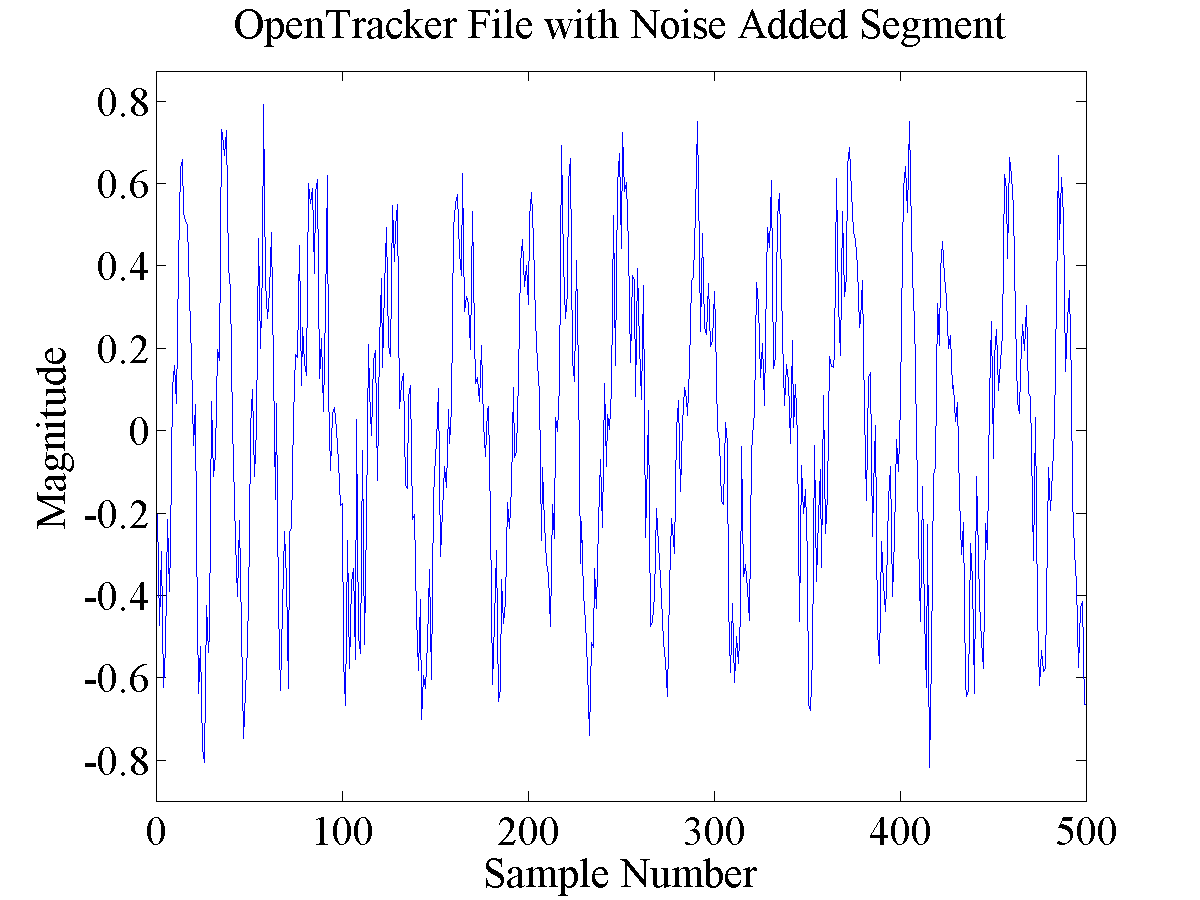
\includegraphics[width=0.75\linewidth]{images/OpenTrackerFilewithNoiseAddedSegment.png} 
	\caption{Example of a generated AFSK signal with artificial white noise added.}
   \label{OT3TestwNoiseSegment}
\end{figure}
 
\section{Los Angeles APRS Test Recordings}
%:04-25:45 57/min averaging over the first 3 minutes
This next benchmark is the de-facto benchmark for APRS modems. The idea behind it is simple, yet it provides a very comprehensive test. The author of this file recorded on air APRS traffic in the Los Angeles Area for 45 minutes. He then removed segments of no traffic and condensed 45 minutes of live recording down to about 25 minutes\,\cite{Smith2009}. This recording is relevant because it is real traffic which contains all of the real life situations including stations close to the receiver, far from the receiver, moving, stationary, different transmit power levels, different hardware, and varying content just to name a few. One disadvantage is that since it is just a random recording of traffic on the air, there is no definitive answer of how many packets are in the file. After listening to the audio file by ear it is approximated that there are a total of about 1463 packets by listening to the first 3 minutes as a sample and extrapolating to the length of the audio segment. This is considered \textit{the} file use for benchmarking in the community and when people discuss the performance of their demodulator, they quote it in how many packets they were able to successfully decode out of this file. An example segment from this off air recording of APRS traffic can be seen in Figure \ref{Track1Segment}. This is just one of the audio files on this author's test CD and is in fact the first one on the CD, so it will be referred to as Track 1. This was the the file that was most important to the testing, but the author also has a second version of this file in Track 2. The only difference between Track 1 and Track 2 is that an audio filter was used to create Track 2 which had the result of being a deemphasized version of Track 1. A quick note about Track 2 is that the processing performed to create it had other undesirable side effects including the white noise between packets being at a much higher magnitude than the packets themselves.
\begin{figure}
  \centering
	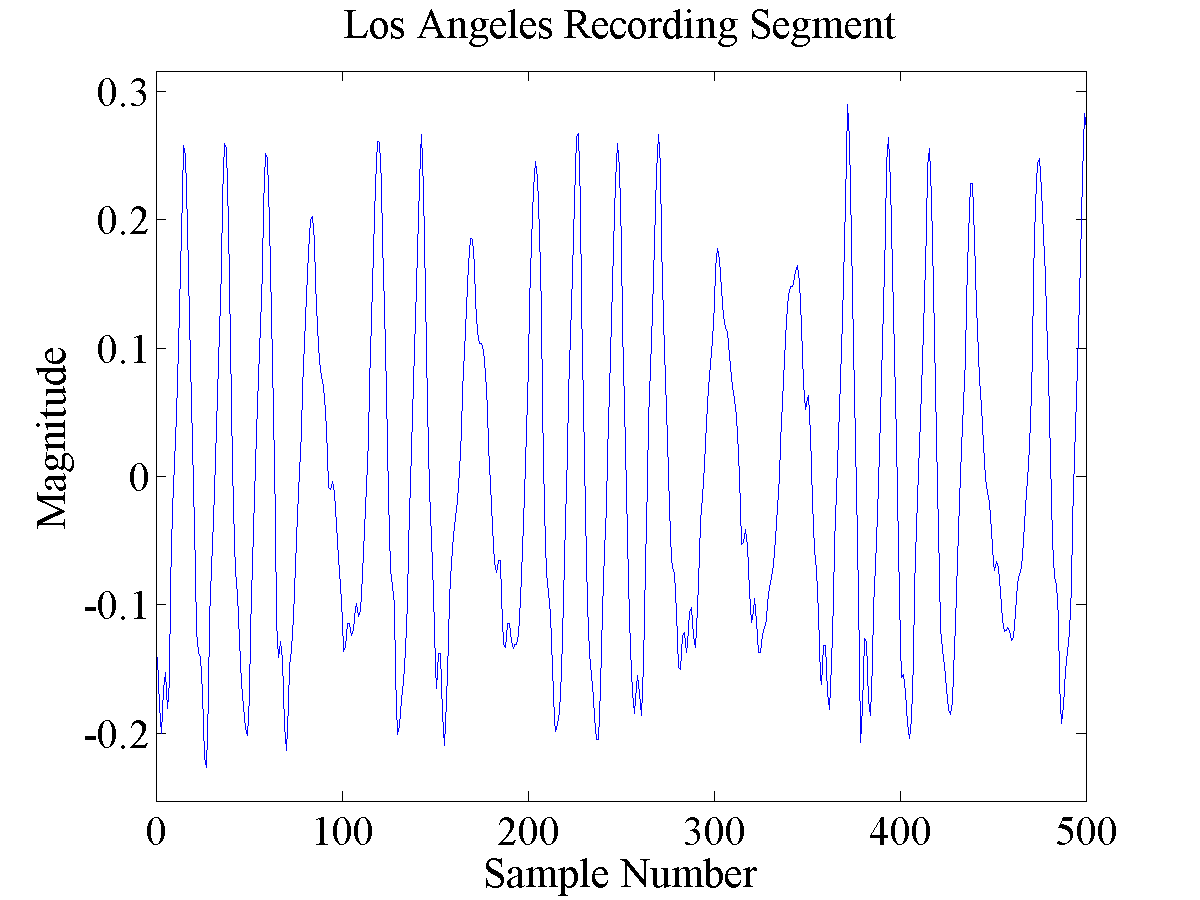
\includegraphics[width=0.75\linewidth]{images/LosAngelesRecordingSegment.png} 
	\caption{Example of the AFSK signal in Track 1 of the Los Angeles Recording Test File.}
   \label{Track1Segment}
\end{figure}
